\documentclass{article}
\usepackage[czech]{babel}
\usepackage[utf8]{inputenc}
\usepackage{graphicx}
\usepackage{pdfpages}
\usepackage{textgreek}
\usepackage{xargs} 
\usepackage{xcolor}
\usepackage{pdfpages}
\usepackage[colorinlistoftodos,prependcaption,textsize=tiny]{todonotes}
\newcommandx{\xtodo}[2][1=]{\todo[linecolor=red,backgroundcolor=red!25,bordercolor=red,#1]{#2}}


\usepackage{listings}
\usepackage{color}

\definecolor{dkgreen}{rgb}{0,0.6,0}
\definecolor{gray}{rgb}{0.5,0.5,0.5}
\definecolor{mauve}{rgb}{0.58,0,0.82}
\definecolor{pblue}{rgb}{0.13,0.13,1}
\definecolor{pgreen}{rgb}{0,0.5,0}
\definecolor{pred}{rgb}{0.9,0,0}
\definecolor{pgrey}{rgb}{0.46,0.45,0.48}


\lstset{frame=tb,
	language=Sql,
	aboveskip=3mm,
	belowskip=3mm,
	showstringspaces=false,
	columns=flexible,
	basicstyle={\small\ttfamily},
	numbers=none,
	numberstyle=\tiny\color{gray},
	keywordstyle=\color{blue},
	commentstyle=\color{dkgreen},
	stringstyle=\color{mauve},
	breaklines=true,
	breakatwhitespace=true,
	tabsize=3
}

\lstset{language=Java,
	showspaces=false,
	showtabs=false,
	breaklines=true,
	showstringspaces=false,
	breakatwhitespace=true,
	commentstyle=\color{pgreen},
	keywordstyle=\color{pblue},
	stringstyle=\color{pred},
	basicstyle=\ttfamily,
	moredelim=[il][\textcolor{pgrey}]{$$},
	moredelim=[is][\textcolor{pgrey}]{\%\%}{\%\%}
}




\begin{document}
	
	
	%---------------------------------------------------------------------------------------------------------------------------------------------------------------%
	
	
	\begin{titlepage}	
		\begin{center}
			
\includegraphics[width=5cm]{logo.jpg}\\[3.5cm]
			{\Huge KIV/VSS}\\[0.5cm]
			{\Large 1.9. – Generování náhodných čísel}\\[0.5cm]
			{\large  Gaussovské rozdělení}\\[4.5cm]
			{\large  Miroslav Liška – A17N0081P}\\[0.5cm]
			{\large  topiker@students.zcu.cz}\\[0.5cm]
			{\large   9.12.1992}\\[0.5cm]
			\vfill
			
			{\large \today}
			
		\end{center}
	\end{titlepage}
	
	
	
	\section{Zadání} %%%%%%%%%%%%%%%%%%%%%%%%%%%%%%%%%%%%%%%%%%%%%%%%%%%%%%%%%%%%%%%%%%%%%%%%%%%%%%%%%%%%%%%%%%%%%%%%%%%%%%%%%%%%%%%%%%%%%%%%%%%%%%%%%%%%%%%%%%
	\setcounter{page}{1}
	
	\subsection{Teoretické pozadí}
	Zejména při fyzické aktivitě nebo příjmu potravy dochází k výrazné změně koncentrace glukózy.
	V zadaných datech máte několik měření koncentrací glukózy v intersticiální tekutině [mmol/l].
	Jsou vzorkovaná po 5 minutách tzv. systémem CGMS. 
	U každého měření je časová značka a měření jsou rozdělena do segmentů, které trvají od několika hodin do několika dní. 
	Vaším úkolem je identifikovat cca 3 - 5 významných kolísání koncentrací glukózy během dne (uvažuje se 3 jídlo a 2 fyzická zátěž). 
	Při identifikaci si můžete pomoci i časovými značkami, případně naměřenou koncentrací v krvi, která by po jídle a při fyzické aktivitě měla být taktéž zvýšená.
	
	V běžném životě si pacient údaje o jídle a fyzické aktivitě zadává manuálně a ještě s chybou. 
	Systém automatické detekce by tuto chybu redukoval a napomohl tak lepší léčbě pacienta. 
	Práce tedy není "šuplíková", ale má praktické využití (cca každý 11. člověk má diabetes a polovina z nich o tom ani neví, protože diabetes nebolí, dokud není pozdě).
	
	Změny koncentrace glukózy lze nejjednoduššeji detekovat jako ohodnocené plovoucí okno - tj. fixní časový úsek, který bude "plout" v čase segmentu od jeho počátku až na konec.
	Ohodnocení okna může být součet rozdílů koncentrací glukózy v daném okně.
	S algoritmem lze dále experimentovat, např. velikost okna a mezní ohodnocení (tj. od kdy je okno považováno za významnou změnu koncentrace glukózy) lze určovat např. pomocí Diferenciální evoluce, nebo jiným algoritmem - může to být i 2D půlení intervalu. 
	Vlastní invenci při vývoji detekčníh algoritmu se meze nekladou.
	
	\subsection{Verze úlohy}
	Zpracujte úlohu alespoň ve dvou verzích ze tří možných:
	
	\begin{itemize}  
		\item Paralelní program pro systém se sdílenou pamětí
		\item x86 CPU + OpenCL/C++ AMP GPGPU
		\item Paralelní program pro systém s distribuovanou pamětí
	\end{itemize}
	
	
	\subsection{Data}
	%%%%%%%%%%%%%%%%%%%%%%%%%%%%%%%%%%%%%%%%%%%%%%%%%%%%%%%%%%%%%%%%%%%%%%%%%%%%%%%%%%%%%%%%%%%%%%%%%%%%%%%%%%%%%%%%%%%%%%%%%%%%%%%%%%%%%%%%%%
	Naměřené hodnoty jsou uloženy ve formátu SQLite verze 3.
	Konkrétně jsou uloženy v tabulce measuredvalue. 
	Požadované hodnoty najdete ve sloupci ist, který vyjadřuje koncetraci v intersticiální tekutině v [mmol/l]. 
	Čas měření je zanesen ve sloupci measuredat, a je ve formátu ISO 8601. Data jsou seskupena do tzv. segmentů, viz  sloupec segmentid. 
	Naměřená data zpracovávejte vždy po celých segmentech. 
	Jméno segmentu lze dohledat  v tabulce timesegment a jméno pacienta analogicky v tabulce subject.
	
	\subsection{Výstup}
	%%%%%%%%%%%%%%%%%%%%%%%%%%%%%%%%%%%%%%%%%%%%%%%%%%%%%%%%%%%%%%%%%%%%%%%%%%%%%%%%%%%%%%%%%%%%%%%%%%%%%%%%%%%%%%%%%%%%%%%%%%%%%%%%%%%%%%%%%%
	Na stdout vypište získané statistické ukazatele jako tabulku v csv formátu. 
	Zároveň vygenerujte grafický výstup ve formátu SVG (pro každý segment jedno SVG), ve kterém graficky znázorníte změny koncentrace glukózy považované za příjem potravy, fyzickou aktivitu, apod. 
	Implentujte přepínač, který buď segment vykreslí v celé jeho délce, anebo ho bude zalamovat po 24 hodinách - tj. osa X (čas) bude mít hodnoty od 00:00 do 23:59. 
	V takovém případě by mohlo být vidět, např. zda pacient snídán či večeří pravidelně - což je také možná nápověda pro detekční algoritmus.
	
	\subsection{Další statistiky}
	%%%%%%%%%%%%%%%%%%%%%%%%%%%%%%%%%%%%%%%%%%%%%%%%%%%%%%%%%%%%%%%%%%%%%%%%%%%%%%%%%%%%%%%%%%%%%%%%%%%%%%%%%%%%%%%%%%%%%%%%%%%%%%%%%%%%%%%%%%
	Program také spusťte s jedním vláknem/procesem a změřte čas výpočtu sériovým kódem a čas výpočtu paralelizovaným kódem (pro všechny verze paralelizovaného kódu zvlášť). 
	Z těchto hodnot vypočítejte následující ukazatele:
	
	\begin{itemize}  
		\item Amdahlův zákon, $f$ -- čas sériově prováděné části kódu
		\item Gustafsonův zákon, $a$ -- část kódu, kterou nelze paralelizovat
		\item Karp-Flattova metrika, $e$ -- část sériově prováděného kódu
	\end{itemize}
	\newpage
	\section{Analýza}
	%%%%%%%%%%%%%%%%%%%%%%%%%%%%%%%%%%%%%%%%%%%%%%%%%%%%%%%%%%%%%%%%%%%%%%%%%%%%%%%%%%%%%%%%%%%%%%%%%%%%%%%%%%%%%%%%%%%%%%%%%%%%%%%%%%%%%%%%%%
	\subsection{Detekce změn koncentrace glukózy}
	O chování koncentrace glukózy v krvi víme (informace z přednášek), že pokud pozorovaný subjekt zkonzumuje nějakou potravinu, konentrace vzroste. 
	Pokud je subjektem vynaložena nějaká aktivita, koncentrace typicky mírně vzroste a pak začne klesat. Tyto akty pak v datech generují významné kolísání, jejichž detekce je cílem práce. Dále je z přednášky známo, že kolísání trvá typicky tři hodiny s tím, že nárůst trvá hodinu a následné klesání pak dvě hodiny. 
	
	Jedním z možných řešení detekce je nalezení lokálních extrémů. Následně se pro každý extrém vezmou spojitě data začínající před extrémem a po extrému o nějaké velikosti. Pro výběr nejlepších výsledků je nutné získané intervaly ohodnotit. Dále je potřeba nějakým způsobem naložit s překrývajícími se intervaly, například jejich sloučením či vyřazením horšího.
	
	Dalším řešením může být evoluční genetický algoritmus. 
	Data jsou rozdělena náhodně na intervaly o pevné velikosti a pro každý interval je vypočítána jeho fitness funkce. Následně se vybrané intervaly posunou a spočítá se jejich fitness funkce a tím vznikne nová generace intervalů. Podle chování genetického algoritmu se s novou generací patřičně naloží. Posouvání probíhá do té doby, dokud nevznikne nejlepší generace intervalů, které jsou pak detekovaným kolísáním.
	
	\subsubsection{Zvolené řešení}
	\label{sec:zvoleneReseni}
	Pro detekci kolísání jsem se rozhodl použít algoritmus posuvného okénka. Princip spočívá v tom, že se napříč daty iteruje tzv. okénkem o velikosti n. Každá iterace posune okénko o jedno měření dál. Každé okénko je ohodnoceno funkcí. 
	V implementaci je jako funkce zvoleno rozdíl sousedních hodnot na druhou. 
	Na druhou z toho důvodu, aby nebylo okénko ohodnoceno záporně. 
	
	Jakmile je spočítáno ohodnocení všech okének, je potřeba vybrat pouze ty nejlepší a nějakým způsobem naložit s okénkami, které se překrývají. Při výběru významějších okének jsem se rozhodl vybrat pouze ty, jejichž ohodnocení je lepší, než průměrná hodnota.
	Po výběru významějších okének je možné, že se budou jednotlivé intervaly překrývat. Je předpokladem, že ve vybraná okénka budou reprezentovat části s významným klesáním či nárůstem. Pokud se tedy intervaly překrývají, je vhodné je spojit. Pro takto spojená okénka znovu spočítáme jejich ohodnocení a následně se vezme n nejlepších.
	\subsection{Načtení uložených dat}
	
	Naměřené hodnoty jsou ve formátu SQLite verze 3. Pro přístup k datům je tedy vhodné přistoupit za pomocí SQL dotazů. Při analýze bylo zjištěno, že ne všechny segmenty uvedené v tabulce segmentů mají i naměřená data a naopak nějaká naměřená data mají id segmentu, které není v tabulce segmentů. Při načtení dat z databáze budou tedy zvolena pouze ta data, jejichž id segmentu odpovídá tabulce segmentů.
	Pro práci hledání kolísání bude nutné, aby data byla seřazena podle data měření (measuredate). Datum měření je uloženo ve formátu ISO 8601. Podle doporučení je dobré převést datum na formát, kdy hodnota 1.0 představuje datum 1.1.1900.
	\subsection{Paralelizace}
	 Na obrázku \ref{fig:flowdiagram} je možné vidět průběh výpočtu a interakcí programu. Slovně byl popsán v sekci \ref{sec:zvoleneReseni}
	 
	Pro parelelizaci této úlohy jsem si vybral paralelizaci se sdílenou pamětí a paralelizaci na GPGPU.
	
	Pravděpodobně nejlepším řešením bude paralelizace na úrovni segmentů, tedy detekce kolísání jednotlivých segmentů bude probíhat současně. Důvodem výběru tohoto místa je, že se jedná o práci s větším množstvím nezávislých dat, tedy by režie spojená s paralelizací nemusel být zpomalující.
	Další možností paralelizace je paralelizace uvnitř segmentu na úrovni jednotlivých dní. Jednalo by se tak o paralelizaci uvnitř paralelizace (segment a jednotlivé dny). Vzhledem k tomu, že počet dat uvnitř jednotlivých dní je nízký (maximálně několik stovek), je předpokladem, že tato paralelizace přínos nepřinese. Tento přístup ale bude v rámci experimentu implementován.
	
	Vzhledem k charakteru zvoleného algoritmu (mnoho podmínek, porovnávání) a obecně nízkému počtu dat, se kterými se provádí matematické operace, je předpokladem, že paralelizace na GPGPU bude spíše zdržující.
	
	
	\begin{figure}
		\centering
		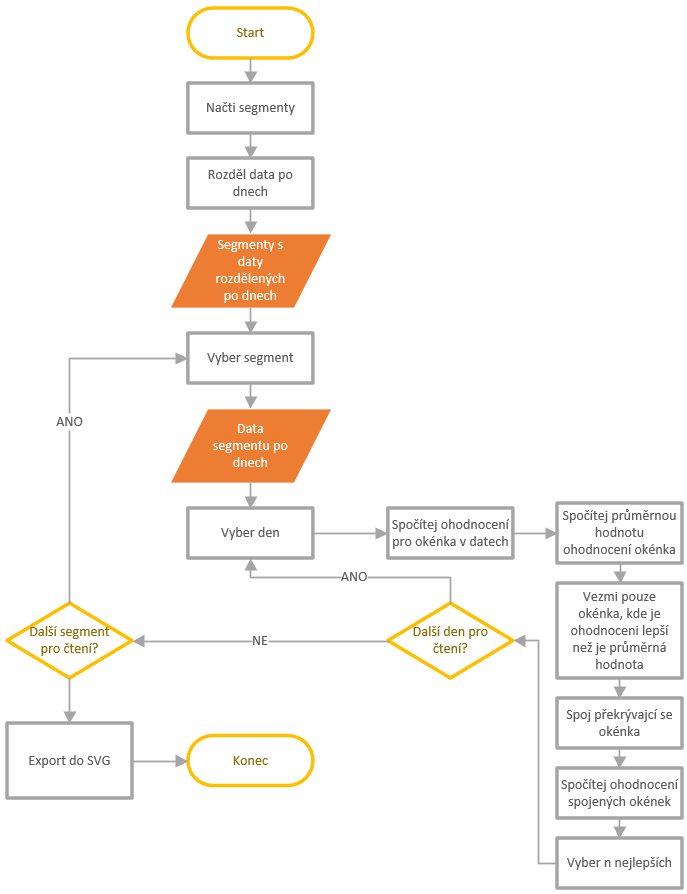
\includegraphics[width=0.7\linewidth]{flowDiagram}
		\caption[Flowdiagram programu]{Flowdiagram programu}
		\label{fig:flowdiagram}
	\end{figure}
	\newpage
	\section{Programátorská dokumentace}
	%%%%%%%%%%%%%%%%%%%%%%%%%%%%%%%%%%%%%%%%%%%%%%%%%%%%%%%%%%%%%%%%%%%%%%%%%%%%%%%%%%%%%%%%%%%%%%%%%%%%%%%%%%%%%%%%%%%%%%%%%%%%%%%%%%%%%%%%%%
	V této kapitole bude popsána implementace programu řešícího zadanou úlohu. Popsány budou především důležité části programu. 
	Program byl naprogramován v jazyce \texttt{C/C++} a byl vyvýjen v prostřední MS Visual Studio 2017. V rámci práce s pamětí byly využity smart pointery, získávaná data jsou reprezentována objekty. Při implementaci jsem využil verzovací systém Git.
	\subsection{Struktura zdrojových souborů}
	
	Zdrojové soubory jsou umístěny v adresáři LISKA\_PPR. Zdrojové soubory jsou pak rozdělené logicky ještě do dalších složek podle funkcionality (Načítání vstupu, dat, hledání kolísání, export). Ve složce sqlLite jsou pak umístěny hlavičkové soubory knihovny SQLite. V této složce jsou také knihovny, které jsou potřebné programu a po překladu jsou nakopírované do patřičných složek.
	
	\subsection{Použité knihovny}
	Pro práci se vstupními daty byla využita \texttt{SQLIte C/C++ Interface}, která umožňuje zadávat SQL dotazy nad jednotlivými tabulkami. Pro paralelizace pak bylo využito knihovny  \texttt{TBB - Thread Building Blocks}, která je implicitně součástí \texttt{Intel Parallel Studio}. Pro paralelizaci na GPGPU bylo využito standardní knihovny AMP.
	
	\subsection{Spuštění aplikace}
	
	Zahájení aplikace probíhá v metodě \texttt{main()} v souboru \texttt{Main.cpp}. Po spuštění programu jsou vstupní parametry předány k parsování třídě \texttt{InputParser}. Pokud jsou vsechny parametry zadány korektně, je zahájen výpočet podle přepínače ve funkci \texttt{runSolution()}
	
	\subsection{Načtění dat}
	Načítání dat je implementováno v souboru \texttt{DataLoader.cpp}. Třída \texttt{DataLoader} obsahuje funkce a procedury, jak pro načtení dat z databáze, tak i jejich předzpracování, jako je nahrazení \texttt{NULL} hodnot. Pro načtení dat z databáze je zde využíváno funkcí knihovny \texttt{SQLIte C/C++ Interface}. Program očekává strukturu zmíněnou v zadání úlohy. Jedna naměřená jednotka je uložena ve třídě \texttt{TMEasuredValue}, kde se čas uložený v databázi přepočítává na čas, kterému rozumí běžný člověk. Naměřené jednotky konkrétního segmentu a dne pak tvoří data pro objekt \texttt{SegmentDay}. Dny pro konkrétní \texttt{Segment} jsou pak uloženy v objektu \texttt{SegmentDays}. Tímto způsobem jsou tedy data hierarchicky poskládána v objektu \texttt{Segment}. Struktura je popsána na obrázku \ref{fig:uml}
	\begin{figure}
		\centering
		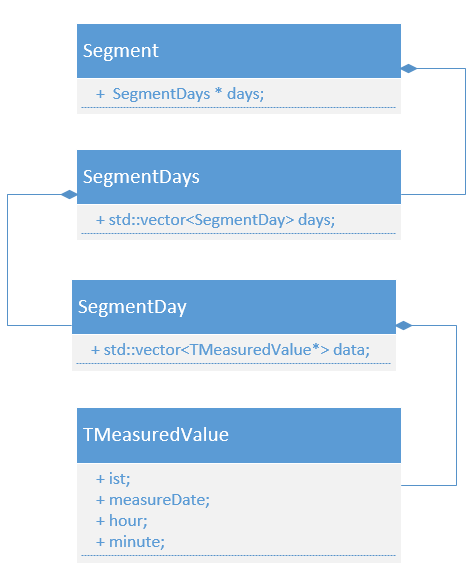
\includegraphics[width=0.7\linewidth]{UML}
		\caption[Hierarchie načtených dat]{Hierarchie načtených dat}
		\label{fig:uml}
	\end{figure}
	
	\subsection{Hledání výkyvů}
	Algoritmus je vizualizován na obrázku \ref{fig:flowdiagram}. 
	
	Program byl nejprve naimplementován sériově a pak zparalelizován s využitím TBB. Jako poslední příšla na řadu paralelizace s využitím AMP. Vzhledem k tomu, že ve funkcích či metodách označených jako \texttt{restrict (amp)} jsou určitá omezení, jako např. absence pointerů, tříd a šablon, bylo nutné celou implementaci provést dvakrát.
	
	Implementace pro procesor je tedy v souboru \texttt{PeakDetector.cpp} a amp implementace je v souboru \texttt{PeakDetectorAMP.cpp}. Parametry funkci zahajuji vypocet jsou ale totozna. Jedna se o velikost okénka, vstupní data a ukazatel na vektor objektů \texttt{Peak}, do kterého se vrací nalezená kolísání, rozdělená po dnech segmentů. Pokud je tedy segment tvořen 3 mi dny, je v kolekci odchylek na stejném indexu, jako je uložen segment, uložena kolekce o velikosti 3, kde je každá kolekce tvořena nalezenými kolísáními.
	
	Implementace detekce v \texttt{PeakDetector.cpp} a  \texttt{PeakDetectorAMP.cpp} je pak co se týče výsledků totožná. Liší se použitými strukturami jednotlivých funkcí.
	
	\subsubsection{Paralelizace na CPU}
	
	Pro paralelizace na úrovni jader procesoru byla použita knihovna \texttt{TBB - Thread Building Block}. 
	Níže můžeme vidět konstrukci \texttt{tbb::parallel\_for()}, která kód vepsaný uvnitř zparalelizuje. Je nutné zajistit zabránění konkurenčnímu zápisu ve sdílené proměnné, typicky že vlákno přistupuje k indexu v poli jako jedinné.
	
	Implementace paralelizace v rámci CPU je realizovaná v rámci segmentů a navíc v rámci jednotlivých dní (pouze experimentálně). 
	Zde je ukázka paralelizace s využitím TBB.
	\vspace{0.4cm}
	\noindent
	\begin{minipage}{\linewidth}
	\begin{lstlisting}[label={lst:parallelFor}]
	tbb::parallel_for(1,128,1,[=](int i){
		//Paralelni vypocet
	}
	\end{lstlisting} 
	\end{minipage}
	
	\subsubsection{Paralelizace na GPGPU}
	Pro paralelizaci na GPGPU jsem použil knihovnu \texttt{C++ AMP}. 
	Implementace je je totožná jako u CPU, nicméně před samotným výpočtem je nutné data zkopírovat do paměti grafiky, k čemuž se používá třída \texttt{concurrency::array\_view<>}, která namapuje data do paměti GPGPU. 
	Po dokončení výpočtu je potřeba zavolat metodu \texttt{synchronize()}, která vypropaguje změnu dat do pole v paměti.
	Zde je ukázka paralelizace na GPGPU. 
	
	\begin{minipage}{\linewidth}
	\begin{lstlisting}[label={lst:ampPara}]
	//pole s hodnotami
	std::vector<int> data;
	
	... //naplneni pole data daty
	
	//namapovani do pameti gpu
	concurrency::array_view<int> data_view(data.size(), data.get());
	
	//Amp parallel foreach
	concurrency::parallel_for_each(data_view.extent, [=](concurrency::index<1> idx) restrict(amp)
	{
		//vypocet paralelne
	}
	//vypropagovani dat mimo GPGPU 
	data_view.synchronize();
	\end{lstlisting} 
	\end{minipage}
	
	\subsection{Vykreslení grafu}
	Vykreslení grafu probíhá, až když jsou všechna kolísání spočítána.
	Pro vykresleni grafu slouží třída \texttt{SVGExporter}, která podle přepínače vykreslí data do jednoho grafu, nebo data podle dní vykreslí do více grafů tak, že graf začíná v čase 0:00 a končí v čase 23:59. Výstup pak uloží do souboru [segment\_číslo segmentu.svg]. Jednotlivá kolísání jsou pak do stejných grafů zaznamenána taktéž.
	
	\begin{figure}[ht!]
	\centering
	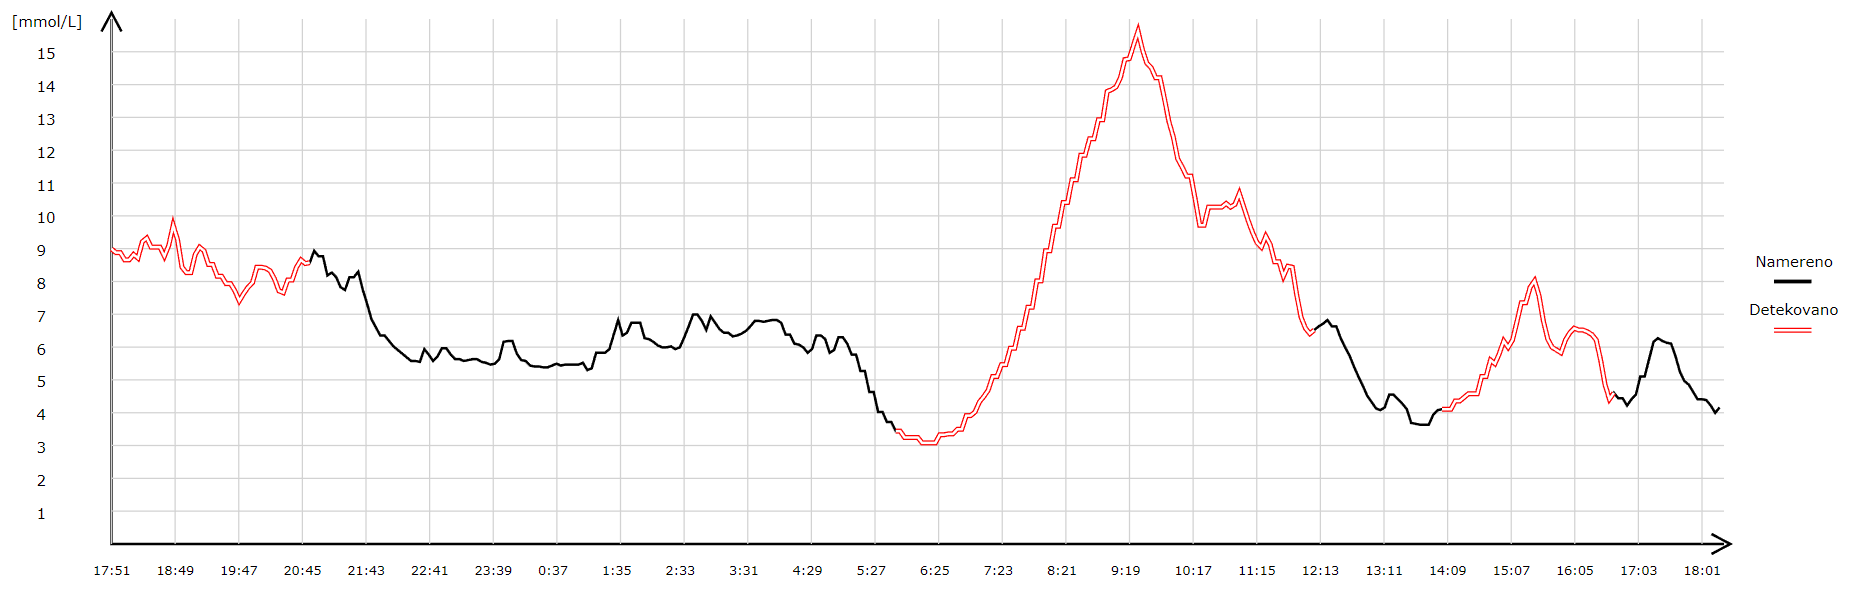
\includegraphics[width=1.0\linewidth]{ukazkaGrafu}
	\caption[Ukázka vykresleného grafu]{Ukázka vykresleného grafu}
	\label{fig:ukazkagrafu}
	\end{figure}
	
	\section{Získané výsledky}
	\label{chap:zhodnoceni}
	\par Testování a výpočty jsem prováděl na stolním počítači s procesorem \texttt{Intel Core i5-6500 @ 3,20GHz}, operační pamětí \texttt{RAM 16,0 GB}, s grafickou kartou \texttt{AMD RADEON R9 380 series 4 GB} a na operečním systému \texttt{Windows 10 64-bit}.
	
	\section{Doby běhů}
	Měření jsem provedl pro každou možnost (sériově, paralelně na úrovni segmentu, paralelně na úrovni segmentu a dne, GPGPU na úrovni segmentů) 1000 krát a časy jsem zprůměroval.
	Výsledné zprůměrované časy můžeme vidět v tabulce \ref{tab:runtime}, časy v tabulce jsou uvedeny v $m s$ (milisekundách).
	\par Spolu s celkovou dobou jsem měřil i doby běhu paralelizované části na CPU, které jsou potřebné pro výpočet statistik (Amdahlův zákon). Program byl spuštěn s velikostí okénka 24, bez exportu grafů, a s výpisem do souboru.
	
	
	\begin{table}[h]
	\centering
	\catcode`\-=12
	\def\arraystretch{1.2}
	\begin{tabular}{|c|c|c|c|}
	\hline
	\textbf{Sériově} & \textbf{Paralelně segmenty} &  \textbf{Paralelně segmenty a dny} & \textbf{GPGPU}  \\ \hline
	\hline
	131,21 $m s$    		  & 127,59 $m s$                  & 128,071 $m s$     		  &        202,15 $m s$                   \\ \hline
	
	\end{tabular}
	\caption{Udává průměrné doby běhů, časy jsou uvedeny v $m s$ (milisekundách)}
	\label{tab:runtime}
	\end{table}
	
	
	Na datech můžeme pozorovat, že výpočet na akcelerátoru je zdaleka nejpomalejší. Nejlepšího výsledku dosahuje paralalelizace na úrovni segmentů. Paralelizace na úrovni segmentů a dnů nedopadla o moc hůře. 
	
	\section{Reálné urychlení}
	Reálně urychlení se spočítá podle vztahu \ref{eq:zrychleni}, kde $T_{1}$ je doba běhu sekvenční 
	\par  Z naměřených hodnot můžeme určit reálné urychlení $S$ pro jednotlivé implementace, které je dáno vztahem \ref{eq:zrychleni}, kde $T_{1}$ je doba běhu sekvenční verze programu a $T_{p}$ je doba běhu paralelizovaného kódu
	\begin{equation} 
	S=\frac{T_{1}}{T_{p}}
	\label{eq:zrychleni}
	\end{equation}
	
	\par Pokud je hodnota větší než jedna došlo k urychlení výpočtu pokud menší pak došlo ke zpomalení.
	
	\begin{table}[h]
	\centering
	\catcode`\-=12
	\def\arraystretch{1.2}
	\begin{tabular}{|c|c|c|c|}
	\hline
	\textbf{Paralelně segmenty} &  \textbf{Paralelně segmenty a dny} & \textbf{GPGPU}  \\ \hline
	\hline
	1,03                  & 1,02     		  &        0,65                 \\ \hline
	
	\end{tabular}
	\caption{Udává reálné urychlení jednotlivých verzí paralelizace oproti sekvenčnímu výpočtu}
	\label{tab:zrychleni}
	\end{table}
	
	\par Z tabulky urychlení \ref{tab:zrychleni} můžeme vidět, že urychlení bylo dosaženo v případech paralelizace na úrovni segmentů a na úrovni segmentů a dnů na CPU. Při výpočtu na GPGPU došlo k výraznému zpomalení. Tímto se potvrdila hypotéza, že výpočet na GPGPU není pro tuto úlohu vhodný (málo dat, velká režie, nevhodný algoritmus pro GPU) U dalších výpočtů budu uvažovat, že $P$ je počet procesorů roven 4.
	
	\section{Amdahlův zákon}
	\par Dobu běhu na jednom procesoru (sekvenčního výpočtu) $T_{1}$ si rozdělíme na dvě části podle \ref{eq:sekvencniSys}, kde $t_{s}$ označuje čas výpočtu na části kódu, kterou nelze paralelizovat a $ t_{p}$ čas výpočtu na kódu, který je paralelizovatelný, ale vykonaný sekvenčně. 
	
	\begin{equation} 
	T_{1} = t_{s} + t_{p}   
	\label{eq:sekvencniSys}
	\end{equation}
	
	V ideálním případě pak bude při výpočtu na $P$ procesorech čas výpočtu dán vztahem \ref{eq:paralelCas}.
	\begin{equation} 
	T_{p} = t_{s} + \frac{t_{p}}{P}   
	\label{eq:paralelCas}
	\end{equation}
	
	Po dosazení vyjádřených $T_{1}$ a $T_{p}$ do vztahu \ref{eq:zrychleni} dostaneme Amdahlův zákon \ref{eq:amdahl1}. Pokud si pomocí $f$ označíme poměr času stráveného výpočtem sekvenčí části ku celkovému času dostaneme vzorec \ref{eq:amdahlfce}.
	
	\begin{equation} 
	S=\frac{T_{1}}{T_{p}} = \frac{t_{s} + t_{p} }{t_{s} + \frac{t_{p}}{P}}
	\label{eq:amdahl1}
	\end{equation}
	
	
	\begin{equation} 
	f = \frac{t_{s}}{t_{s} + t_{p}}
	\label{eq:amdahlfce}
	\end{equation}
	
	Dosazením a vyjádřením $f$ do \ref{eq:zrychleni} získáme známější tvar Amdahlova zákona.
	
	\begin{equation} 
	S=\frac{1}{f + \frac{1-f}{P}} \leq  \frac{1}{f}
	\label{eq:amdahl2}
	\end{equation}
	
	Pro výpočet $f$ a $S$ potřebujeme jednotlivé doby $t_{p}$ a $t_{s}$ , které jsou uvedeny v tabulce \ref{tab:dobyBeh2}. Dobu $t_{s}$ získáme odečtením celkové doby běhu z tabulky \ref{tab:runtime} od odpovídajících dob $t_{p}$.
	
	
	\begin{table}[h]
	\centering
	\catcode`\-=12
	\def\arraystretch{1.2}
	\begin{tabular}{|c|c|c|c|}
	\hline
	\textbf{Doba}   & \textbf{Sériově} \\ \hline
	\hline
	$T_{1}$    		  & 131,213 $m s$ \\ \hline
	$t_{p}$                  & 2,81 $m s$  \\ \hline
	$t_{s}$           		  & 128,403 $m s$ \\ \hline
	\end{tabular}
	\caption{Doby běhu programu sekvenčně}
	\label{tab:dobyBeh2}
	\end{table}
	
	Dosazením získaných hodnot do vzorců \ref{eq:amdahlfce} a \ref{eq:amdahl2} (popř. \ref{eq:amdahl1}) získáme požadované statistické údaje $f$ a $S$, které můžeme vidět v tab. \ref{tab:amdahlFinal}.
	
	\begin{table}[h]
	\centering
	\catcode`\-=12
	\def\arraystretch{1.2}
	\begin{tabular}{|c|c|c|c|}
	\hline
	\textbf{}   & \textbf{Sériově} \\ \hline
	\hline
	$f$    		  & $0,979$\\ \hline
	$S$                  &  $1,016$\\ \hline
	\end{tabular}
	\caption{Udává vypočítané hodnoty ukazatelů $f$ a $S$ pro Amdahlův zákon}
	\label{tab:amdahlFinal}
	\end{table}
	
	\section{Gustafsonův zákon}
	Dobu běhu na $P$ procesorech označíme jako $T_{p}$ danou vztahem \ref{eq:dobaBehuGusta}, kterou rozdělíme na dobu běhu paralelní části  $t_{p}^{*}$ a sekvenční části  $t_{s}^{*}$
	
	\begin{equation} 
	T_{p} = t_{s}^{*} + t_{p}^{*} 
	\label{eq:dobaBehuGusta}
	\end{equation}
	
	Doba běhu na jednom procesoru bude dána vzorcem \ref{eq:dobaBehuSekGust}.
	
	\begin{equation} 
	T_{1} = t_{s}^{*} + P \cdot t_{p}^{*} 
	\label{eq:dobaBehuSekGust}
	\end{equation}
	
	Dosazením do vzorce \ref{eq:zrychleni} pro zrychlení dostanem \ref{eq:sgusta}
	
	
	\begin{equation} 
	S=\frac{T_{1}}{T_{p}} = \frac{t_{s}^{*} + P \cdot t_{p}^{*} }{t_{s}^{*} + t_{p}^{*}}
	\label{eq:sgusta}
	\end{equation}
	Opět můžeme vyjádřit $\alpha$ jako poměr času stráveného výpočtem sekvenčnčí části ku celkovému času, ale na paralelním počítači a  dostaneme vzorec \ref{eq:amdahlfce2}.
	
	\begin{equation} 
	\alpha = \frac{t_{s}^{*}}{t_{s}^{*} + t_{p}^{*}}
	\label{eq:amdahlfce2}
	\end{equation}
	
	Zrychlení pak také můžeme zapsat jako \ref{eq:zrychleniGust22}
	
	\begin{equation} 
	S = P - \alpha(P-1)
	\label{eq:zrychleniGust22}
	\end{equation}
	
	Jednotlivé doby $t_{s}^{*}$ a $t_{p}^{*}$ jsou vidět v tabulce \ref{tab:doby3}
	
	\begin{table}[h]
	\centering
	\catcode`\-=12
	\def\arraystretch{1.2}
	\begin{tabular}{|c|c|c|c|}
	\hline
	\textbf{Doba}   & \textbf{TBB segment} & \textbf{TBB segment a den} &  \textbf{Akcelerator} \\ \hline
	\hline
	$T_{p}$    		  & 127,59 $m s$                  & 128,071 $m s$     		  &        202  $m s$                     \\ \hline
	$t_{p}^{*}$                  & 1,16 $m s$                  & 1,26 $m s$               &       61,721 $m s$                         \\ \hline
	$t_{s}^{*}$           		  & 126,43 $m s$                  & 126,81 $m s$                       & 140,279   $m s$          \\ \hline
	\end{tabular}
	\caption{Udává jednotlivé doby běhu paraleně vykonaného programu}
	\label{tab:doby3}
	\end{table}
	
	Dosazením do vzorce \ref{eq:amdahlfce2} a \ref{eq:zrychleniGust22} získáme požadované ukazatele $\alpha$ a $S$, které jsou vypočteny v tabulce \ref{tab:sfgustik}
	
	
	\begin{table}[h]
	\centering
	\catcode`\-=12
	\def\arraystretch{1.2}
	\begin{tabular}{|c|c|c|c|}
	\hline
	\textbf{}   & \textbf{TBB segment} & \textbf{TBB segment a den} &  \textbf{Akcelerator} \\ \hline
	\hline
	$\alpha$    		  & $0,990$                  &  $0,989 $     		  &       $ 0,0766$                     \\ \hline
	$S$                  &  $1,027 $                  &   $1,033$               &      $ 1,702$                         \\ \hline
	\end{tabular}
	\caption{Udává vypočítané hodnoty ukazatelů $\alpha$ a $S$ pro Gustafsonův zákon}
	\label{tab:sfgustik}
	\end{table}
	
	
	\section{Karp-Flattova metrika}
	Karp-Flatovu metriku $e$ je definovaná vzorcem \ref{eq:karpFlat}, kde $P$ je počet procesorů a $\psi$ je urychlení na $P$ procesorech
	
	\begin{equation} 
	e={\frac  {{\frac  {1}{\psi }}-{\frac  {1}{P}}}{1-{\frac  {1}{P}}}}
	\label{eq:karpFlat}
	\end{equation}
	
	Pro výpočet $\psi$ podle \ref{eq:psi} potřebujeme znát $T(p)$, který určíme ze vztahu  \ref{eq:tppsi}, kde $T_{s}$ je doba běhu sekvenční části kódu a  $T_{p}$ je doba běhu paralelizovatelné části sekvenčně. Dále je potřeba určit $T(1)$ podle \ref{eq:tjednapsi}.
	
	
	\begin{equation} 
	\psi = \frac{T(1)}{T(p)}
	\label{eq:psi}
	\end{equation}
	
	\begin{equation} 
	T(p) = T_{s} + \frac{T_{p}}{P}
	\label{eq:tppsi}
	\end{equation}
	
	\begin{equation} 
	T(1) = T_{s} + T_{p}
	\label{eq:tjednapsi}
	\end{equation}
	
	Vypočítané hodnoty lze vidět v tabulce \ref{tab:karpik}, při výpočtu byly použity naměřené hodnoty z \ref{tab:dobyBeh2}
	
	\begin{table}[h]
	\centering
	\catcode`\-=12
	\def\arraystretch{1.2}
	\begin{tabular}{|c|c|c|c|}
	\hline
	\textbf{}   & \textbf{Sériově} \\ \hline
	\hline
	$\psi$    		  & $1,0269$\\ \hline
	$e$                  &  $0,723$\\ \hline
	\end{tabular}
	\caption{Udává vypočítané hodnoty ukazatelů $\psi$ a $e$ pro Karp-Flattovu metriku}
	\label{tab:karpik}
	\end{table}
	

	\section{Uživatelská příručka}
	Pro spuštění aplikace je potřeba mít v PC, na které aplikace poběží, dynamické knihovny pro \texttt{TBB - Thread Building Blocks } a \texttt{SQLLite}. SqlLite je přibalené v rámci odevzdané práce.
	\subsection{Překlad aplikace}
	Aplikace se překládá za využítí vývojového prostředí \texttt{MS Visual Studio 2017}, ve kterém je možné přiložený projekt otevřít. Při překladu bude vývojové prostředí vyžadovat nastavení cest ke knihovnám \texttt{TBB} a \texttt{SQLite}.
	\subsection{Spuštění aplikace}
	Přeložený spustitelný soubor se jmenuje \texttt{LISKA\_PPR.exe}. Aplikaci je možné spustit s využitím vývojového prostředí či z příkazové řádky příkazem \texttt{LISKA\_PPR.exe [PARAMETRY]}. Jednotlivé parametry programu budou popsány v následující podsekci.
	
	Program vypisuje standartní výstup. Data jsou ve formátu CSV a to ve formátu:\newline \texttt{Id segmentu;index dne;hodina zacatku kolisani:minuta zacatku kolisani;\newline hodina konce kolisani:minuta konce kolisani}
	\subsubsection{Parametry programu}
	
	Program vyžaduje dva povinné parametry. Prvním je cesta a název souboru s daty. Druhým parametrem je metoda paralelizace, která má být použita. 
	
	\vspace{0.4cm}
	\noindent
	\begin{minipage}{\linewidth}
	\begin{lstlisting}
	
	Parametry:
	-db [cesta k databazi]
	-method [identifikator par. metody: 1 - seriove, 2 - paralelne na urovni semgnetu, 3 - paralelne na zaklade dnu, 4 - akcelerator]
	-exportPath [kam se ma exportovat svg]
	-window [velikost detekcniho okna]
	-graphPerDay [identifikator zvoleneho grafu: 0 - Segment v jednom grafu, 1 - Co den, to graf]
	
	Ukazka:
	LISKA_PPR.exe -db "direcnet.sqlite" -method 2 -window 24 -graphPerDay 0 -exportPath "/Export"
	\end{lstlisting} 
	\end{minipage}
	
	\section{Závěr} %%%%%%%%%%%%%%%%%%%%%%%%%%%%%%%%%%%%%%%%%%%%%%%%%%%%%%%%%%%%%%%%%%%%%%%%%%%%%%%%%%%%%%%%%%%%%%%%%%%%%%%%%%%%%%%%%%%%%%%%%%%%%%%%%%%%%%%%%%
	Zadání semestrální práce bylo splněno.
	
	Vytvořil jsem program pro detekci kolísání glukózy v naměřených datech.
	Při vypracování úlohy jsem se naučil pracovat se smart pointery, které pro mě byly novinkou a do budoucna je budu určitě využívat. Dále jsem se naučil, jak implementovat paralelizaci s využitím knihovny \texttt{TBB} a jak provádět výpočet na akceleráru s využitím \texttt{C++ AMP}.
	
	Zvolená metoda pro detekci se na zkoumaných datech jeví jako dostačující. Jejími nedostatky je ovšem to, že nedokáže poznat, zda se data ve zkoumaném okně pouze vlní, nebo se významně mění.Tento problém by šel odstranit vyhlazením dat. Na to mi už ale nezbyl čas.
	
	Program by šel rozšířit o další metody detekce kolísání. Zajímavými se mi zdály genetické algoritmy, či nějakým způsobem pracovat s integrály.
	
	
	 
\end{document}